\svnInfo $Id: elision.tex 6891 2007-10-02 06:13:49Z kohlhase $
\svnKeyword $HeadURL: https://svn.omdoc.org/repos/omdoc/projects/omdoc-2.0/OpenMath-paper/elision.tex $
\section{Flexible Elisions}\label{sec:elision}

There are several situations in which it is desirable to display only some parts of the
presentation:
\begin{itemize}
\item Brackets that are redundant due to operator precedences can be omitted.
\item Arguments that are strictly necessary are omitted to simplify the notation, and the
  reader is trusted to fill them in from the context.
\item Arguments are omitted because they have default values. For example $\log_{10}x$ is
  often written as $\log x$.
\item Arguments whose values can be inferred from the other arguments are usually
  omitted. For example, matrix multiplication formally takes five arguments, namely the
  dimensions of the multiplied matrices and the matrices themselves, but only the latter
  two are displayed.
\end{itemize}

Typically, these elisions are confusing for readers who are getting acquainted with a
topic, but become more and more helpful as the reader advances.  For experienced readers
more is elided to focus on relevant material, for beginners representations are more
explicit.  In the process of writing a mathematical document for traditional (print)
media, an author has to decide on the intended audience and design the level of elision
(which need not be constant over the document though). With electronic media we have new
possibilities: we can make elisions flexible. The author still chooses the elision level
for the initial presentation, but the reader can adapt it to her level of competence and
comfort, making details more or less explicit.

To provide this functionality, we give each token in the $w_i$ an integer
{\defemph{visibility level}} and group them into {\defemph{elision groups}}. High
levels mean high elidability. 

\begin{newpart}{@FR/CL, please check, and adapt the examples. This is important stuff, we
    want people to understand it.}
  Brackets form a special elidability group of their own. Assume we calculate $\pres{O}p$
  for an {\openmath} object $O$, and the notation definition chosen to present $O$ has the
  output precedence $q$ and returns the the token string $B$. Then every bracket token in
  $B$ is given the visibility level $d\colon=\max\{q-p,0\}$. Thus brackets where the
  difference between input and output precedence is higher are more elidable because they
  are easier to reconstruct. Brackets with a visibility level 0 are necessary and cannot
  be elided.

  In the special cases where $p$ and $q$ are both positive or both negative infinity, we
  put $p-q$ to be $0$ resulting in these brackets being unelidable. If $O$ is presented as
  a top-level object, i.e., not as the result of a recursive call to the presentation
  procedure, $p$ is assumed to be negative infinity, which means that top-level brackets
  have the highest elidability.
\end{newpart}

\begin{newpart}{@CL/FR: please check this}
  Elision can take various forms in print and digital media. In static media like
  traditional print on paper or the PostScript format, we have to fix the elision level, and
  can decide at presentation time which elidable tokens will be printed and which will
  not. In this case, the presentation algorithm will take visibility thresholds $T_g$ for
  every elidability group $g$ as a user parameter and then elide (i.e. not print) all
  tokens in visibility group $g$ with level $l>T_g$.

  In an output format that is capable of interactively changing its appearance, e.g.
  dynamic XHTML+MathML (i.e. XHTML with embedded Presentation {\mathml} formulas, which
  can be manipulated via {\javascript} in browsers), an application can export the the
  information about elision groups and levels to the target format, and can then
  dynamically change the visibility thresholds by user interaction.

%  \begin{wrapfigure}{r}{8.5cm}\vspace*{-.5cm}
\begin{figure}[ht]\centering
    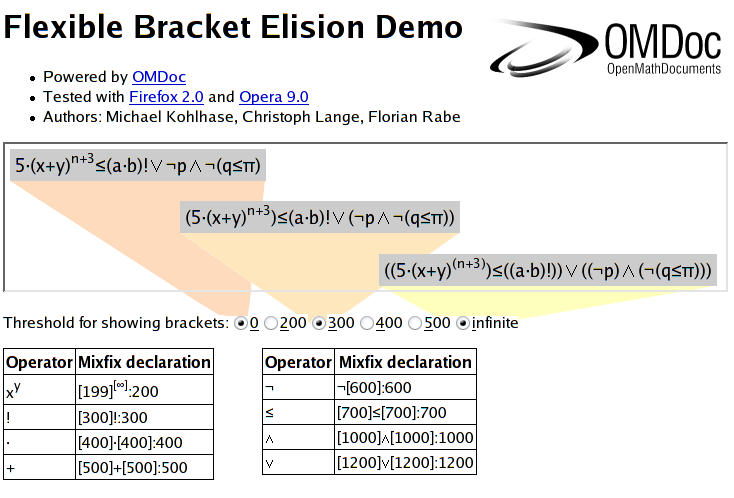
\includegraphics[width=8.5cm]{demo-shot}
    \caption{Flexible Elision of Brackets in XHTML}
    \label{fig:flexible-elision}\vspace*{-.5cm}
\end{figure}
%  \end{wrapfigure}
  We have implemented a prototypical flexible elision scheme for dynamic XHTML, by
  generating tokens for all elidable parts, wrapping them in
  {\element[ns-elt=xhtml]{span}} elements and exporting the elision group and level
  information as XML attributes {\attributeshort[ns-attr=omdoc]{egroup}} and
  {\attributeshort[ns-attr=omdoc]{elevel}} on these elements. All
  {\element[ns-elt=xhtml]{span}} elements with visibility group $g$ and level $l>T_g$ are
  augmented with the attribute {\snippet{style="display:none"}}, which elides them. If the
  user changes the threshold, an embedded {\javascript} function can be used to set the
  display property accordingly. In Figure~\ref{fig:flexible-elision}, we show the system
  with three levels of bracketing thresholds. The same technique would work for
  XHTML+MathML, if the CSS {\tt{display}} directive were implemented for {\mathml}
  elements across browsers. 
\end{newpart}



%%% Local Variables: 
%%% mode: stex
%%% TeX-master: "presel"
%%% fill-column: 90
%%% sentence-end-double-space: nil
%%% End: 

% LocalWords:  FR CL ns elt xhtml attr omdoc egroup elevel stex presel
